%\documentclass[10pt,twocolumn]{article}
\documentclass[sigconf]{acmart}
\acmConference[ESEC/FSE 2018]{The 26th ACM Joint European Software Engineering Conference and Symposium on the Foundations of Software Engineering}{4--9 November, 2018}{Lake Buena Vista, Florida, United States}
% * <trandles@lanl.gov> 2018-06-14T15:27:12.447Z:
%
% ^.
\usepackage{times}
\usepackage{graphicx}
\usepackage{xspace,shortcut}
\usepackage{comment}
\usepackage{color,soul}
\usepackage{tcolorbox}
\tcbuselibrary{skins}
\usepackage{listings}


\lstset
{ %Formatting for code in appendix
    %basicstyle=\footnotesize
    numbers=left,
    %stepnumber=1,
    showstringspaces=false,
    tabsize=1,
    breaklines=true,
    breakatwhitespace=false,
    backgroundcolor=\color{backcolour}
}

\definecolor{backcolour}{rgb}{0.95,0.95,0.92}

\begin{document}

\title{\texttt{BeeSwarm}: Enabling Scalability Tests in Continuous Integration}

\author{Jieyang Chen}
\affiliation{%
  \institution{University of California, Riverside}
}
\email{jchen098@ucr.edu}

\author{Qiang Guan, Paul  Bryant}
\affiliation{%
  \institution{Kent State University}
}
\email{{qguan, pbryant1}@kent.edu}

\author{Li-Ta Lo, Patricia Grubel, and Tim Randles}
\affiliation{%
  \institution{Los Alamos National Laboratory}
}
\email{{ollie, pagrubel, trandles}@lanl.gov}





\begin{abstract}
Testing is one of the most important steps in software development. It ensures the quality of software. Continuous Integration (CI) is a widely used testing system that can report software quality to the developer in a timely manner during the development progress. Performance, especially scalability, is another key factor for High Performance Computing (HPC) applications. Though there are many applications and tools to profile the performance of HPC applications, none of them are integrated in the continuous integration. On the other hand, no current continuous integration tools provide easy-to-use scalability test capabilities.
%However, current CI only tests the software's functionality.  No current CI implementation provide . 
In this work, we propose BeeSwarm, a scalability test system that can be easily applied to the current CI test environment enabling scalability test capability for HPC developers. As a showcase, BeeSwarm is integrated into Travis CI and executes the scalability test workflow on Chameleon cloud. 
%\pat{Do you have a reference for Chameleon?}
%\qguan{This is qguan}

\end{abstract}
\maketitle
\footnotetext[1]{The
publication has been assigned the LANL identifier LA-UR-18-25223.}
\section{Introduction}
High software quality is one of the most important goal of software development. Software testing serves as the most widely used approach to ensure the quality of softwares meet expectation.
%Software testing is one of the most important processes in HPC software development. 
A good way to test software is to include automated tests in the build process.  With the rise of Extreme Programming (XP) and Test Driven Development (TDD), self-testing processes for code development have become popular and are widely adopted by many software development projects. 
As softwares become increasingly structurally complicated, the number of developers involved in the development process increases. As each developer makes progress, they commit their work periodically (every several hours or days) to the central code repository (e.g., git, SVN). Not only does each developer's work require testing, the integration of work between developers also requires testing. So, Continuous Integration (CI) \cite{fowler2006continuous} is widely adopted in many software development projects. A CI server is used dedicatedly for testing. Each time a developer makes a commit of her work to the central code repository, the CI server automatically make a clone of the project and conduct pre-designed tests, so that it can constantly monitor the quality of the software in terms of correctness and report potential problems in a timely fashion, helping developers make bug fixes more efficiently.  %\pat{I wouldn't say the servers mimic the production env.}
%\pat{what is this a hanging here for}

\begin{figure*}[h]
    \centering
    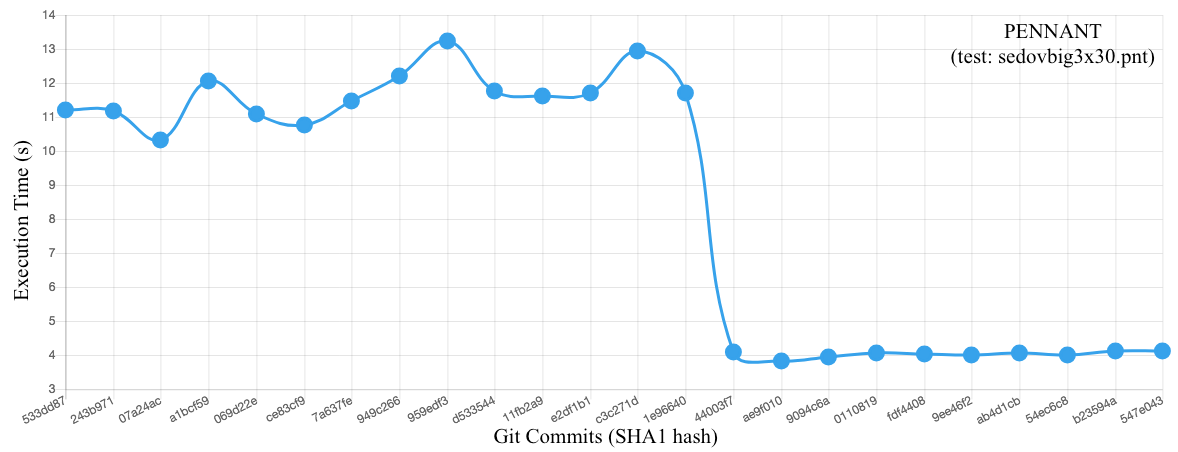
\includegraphics[width=1\textwidth]{figures/CI-motivation-2.png}
    \caption{Example: the performance of Legion \cite{bauer2012legion} changes as developers make progress. The performance is obtained by running a benchmark PENNANT\cite{ferenbaugh2015pennant} on the Legion system. The test suit sedovbig3x30 running on 10 processes (CPU cores) is used. 
%\textcolor{red}{Caption should be changed because this perforamnce is about Legion not PENNANT.}
}
    \label{exp}
\end{figure*}


When it comes to HPC applications, \textit{performance} and \textit{scalability} %large-scale
%\trandles{Remove 'large-scale' here because you have it at the end of the sentence} 
are the other two important factors of software quality besides correctness, since the application are usually designed to deliver high performance on given platforms. Also applications that aim to solve complex time-consuming problems are expected to obtain good speedup when deployed on multi-node clusters, many-core architectures, or large-scale supercomputers. The scalability of HPC application is usually interpreted as how much speed up can be obtained given more computing resources. Better scalability means that the HPC application can use the underlying computing resources more efficiency and constantly deliver good performance on a various amount of computing resources.

During the HPC application development, as developers make progress,
%\pat{not sure if I changed your meaning here}
and they commit their work to the central code repository, the scalability of the application can change. For instance, it can be caused by changes in algorithm design, tunable parameters, and different hardware architectures of target production systems. For example, \textbf{Fig. \ref{exp}} shows the  performance of Legion \cite{bauer2012legion}, a data-centric parallel programming system, changes %\pat{shouldn't you explain what Circuit is I assume it's some sort of simulation, is it really an HPC code or just a benchmark code? Also, the axes of figure need to be labels I have no idea what they are}
%\trandles{Change the data point styles on the graph and refer to them by the symbols instead of colors.  Color-blind readers won't be able to easily distinguish between the two data series as presented.}
with different source code commits. The performance is obtained by running a benchmark software, PENNANT\cite{ferenbaugh2015pennant}, on the Legion system. As we can see the execution time can significantly change as developers make progresses. Receiving performance or scalability results like this in a timely manner can greatly help developers make better decisions about their code design and deliver HPC software with expected quality. However, current designs of CI services are commonly focused on monitoring the software quality in terms of correctness (e.g., detecting software bugs). To the best of our knowledge, none of the current works can easily enable automatic performance or scalability tests in CI since the test environment of CI is usually deployed on a single machine incapable of conducting large-scale scalability test.

\begin{figure}[h]
    \centering
    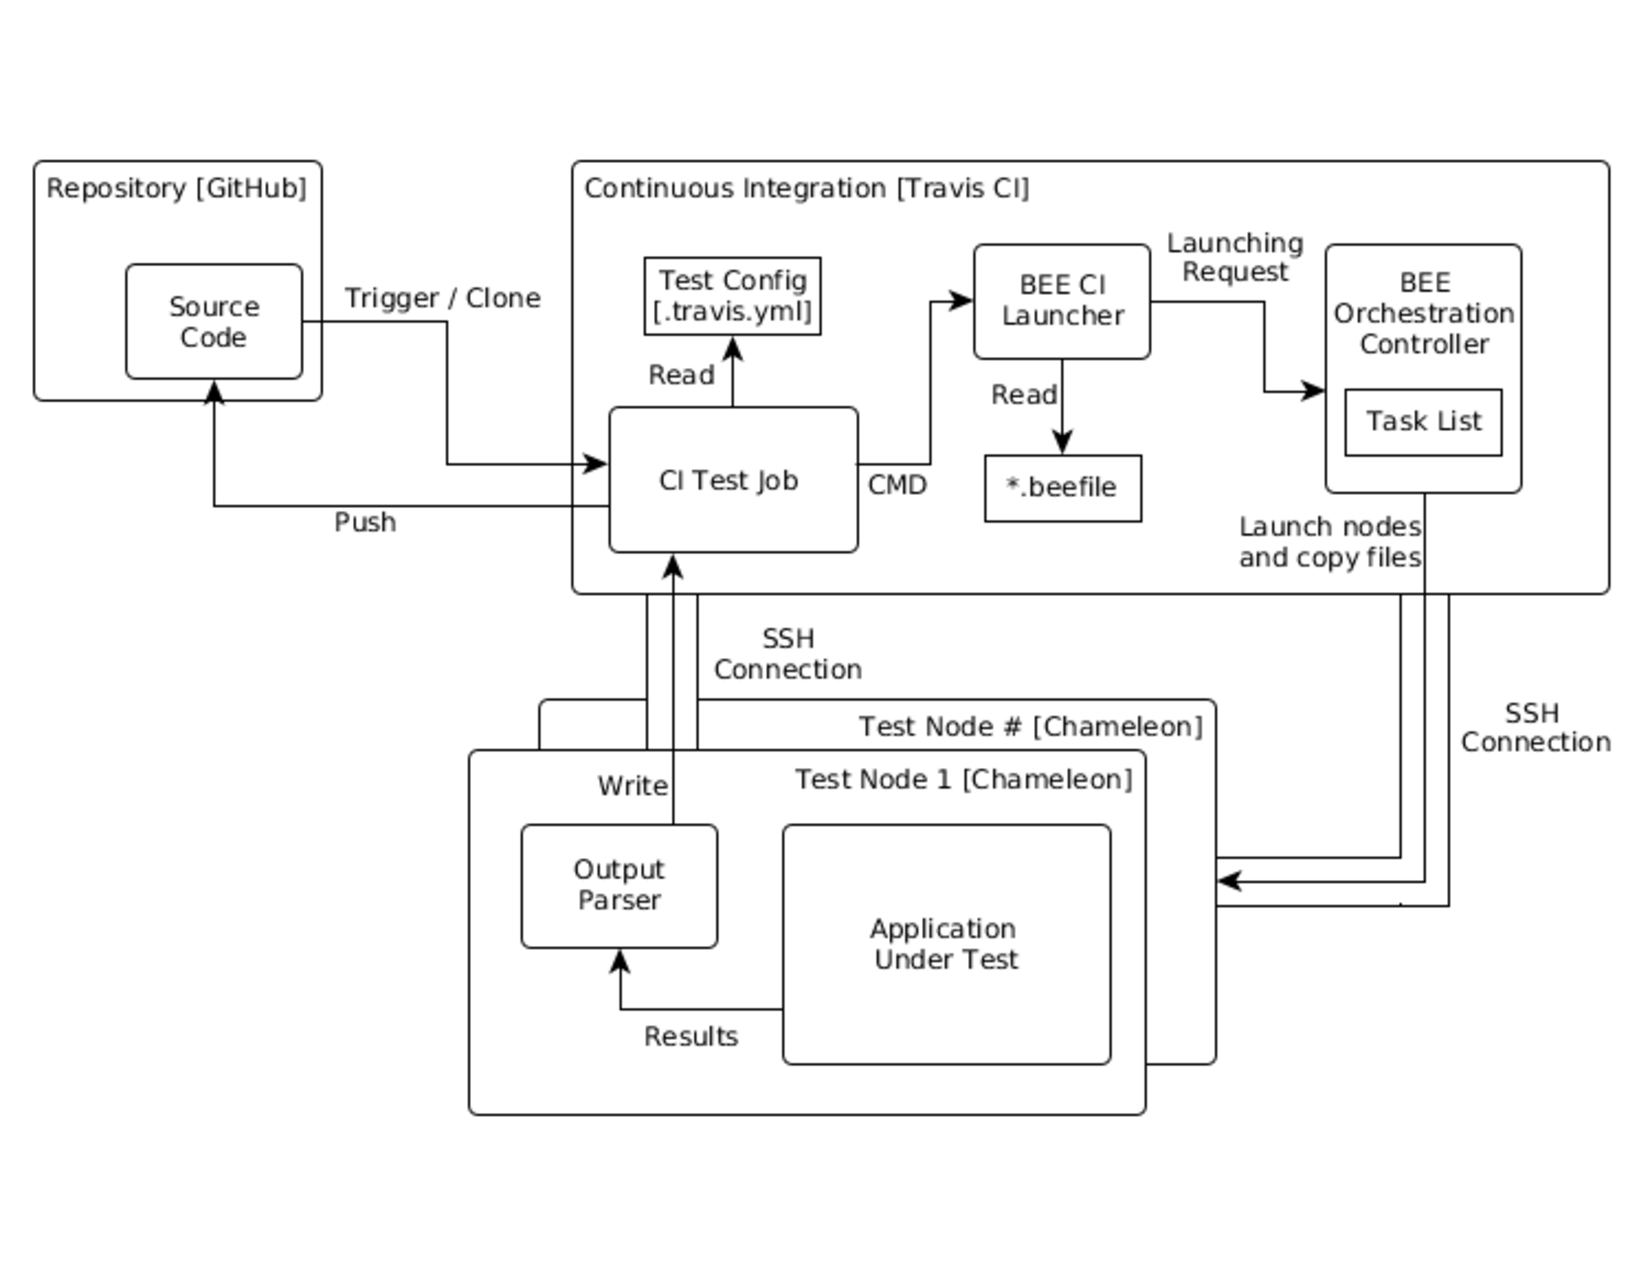
\includegraphics[width=0.5\textwidth]{figures/beeSwarm_Arch_ver02.pdf}
    \caption{Architecture of \texttt{BeeSwarm}. %\textcolor{red}{****Figure is not readable}
    }
    \label{arch}
\end{figure}


In this work, we propose a performance and scalability test system for CI -- \texttt{BeeSwarm}. \texttt{BeeSwarm} can be used as a plug-in for any current CI service. It takes the widely used Docker container as input, and the performance and scalability test can run on both HPC cluster environments and cloud computing environments. Just like the original correctness test in CI, the performance and scalability test are also autonomic. It only requires users to make simple specifications about the test environment they want to use and the test specification they need. Every time developers commit a change to the central code repository, they can choose to schedule a scalability test after the success of original correctness test. The performance and scalability test results will be automatically pushed back to the central code repository. %\pat{can this be controlled, maybe they don't want every change to spawn a scalability test}
Although we deploy \texttt{BeeSwarm} on Travis CI in this work, it can also be deployed on any other CI test environment. To deploy on another CI platform, only minimum modifications to the \texttt{BeeSwarm} configuration scripts are necessary, which makes \texttt{BeeSwarm} highly portable across CI platforms. In addition, although we only show the use of Chameleon cloud, the scalability test can also be executed on any other BEE-supported platform (HPC clusters, AWS, OpenStack, etc). This gives developers the flexibility to choose the platform they want their applications to run on.

The rest of this paper is organized as follows. We motivate our work in section \ref{motivation}. In section \ref{background}, we give necessary background that can help readers understand this work. We provide design details of \texttt{BeeSwarm} in section \ref{design} followed by experimental evaluation in section \ref{experiments}. Section \ref{related_work} discuss recent works that related to ours. Finally, section \ref{conclusion} concludes our work. %\textcolor{red}{Please change this accordingly after adding the motivation session}

\begin{figure*}[h]
    \centering
    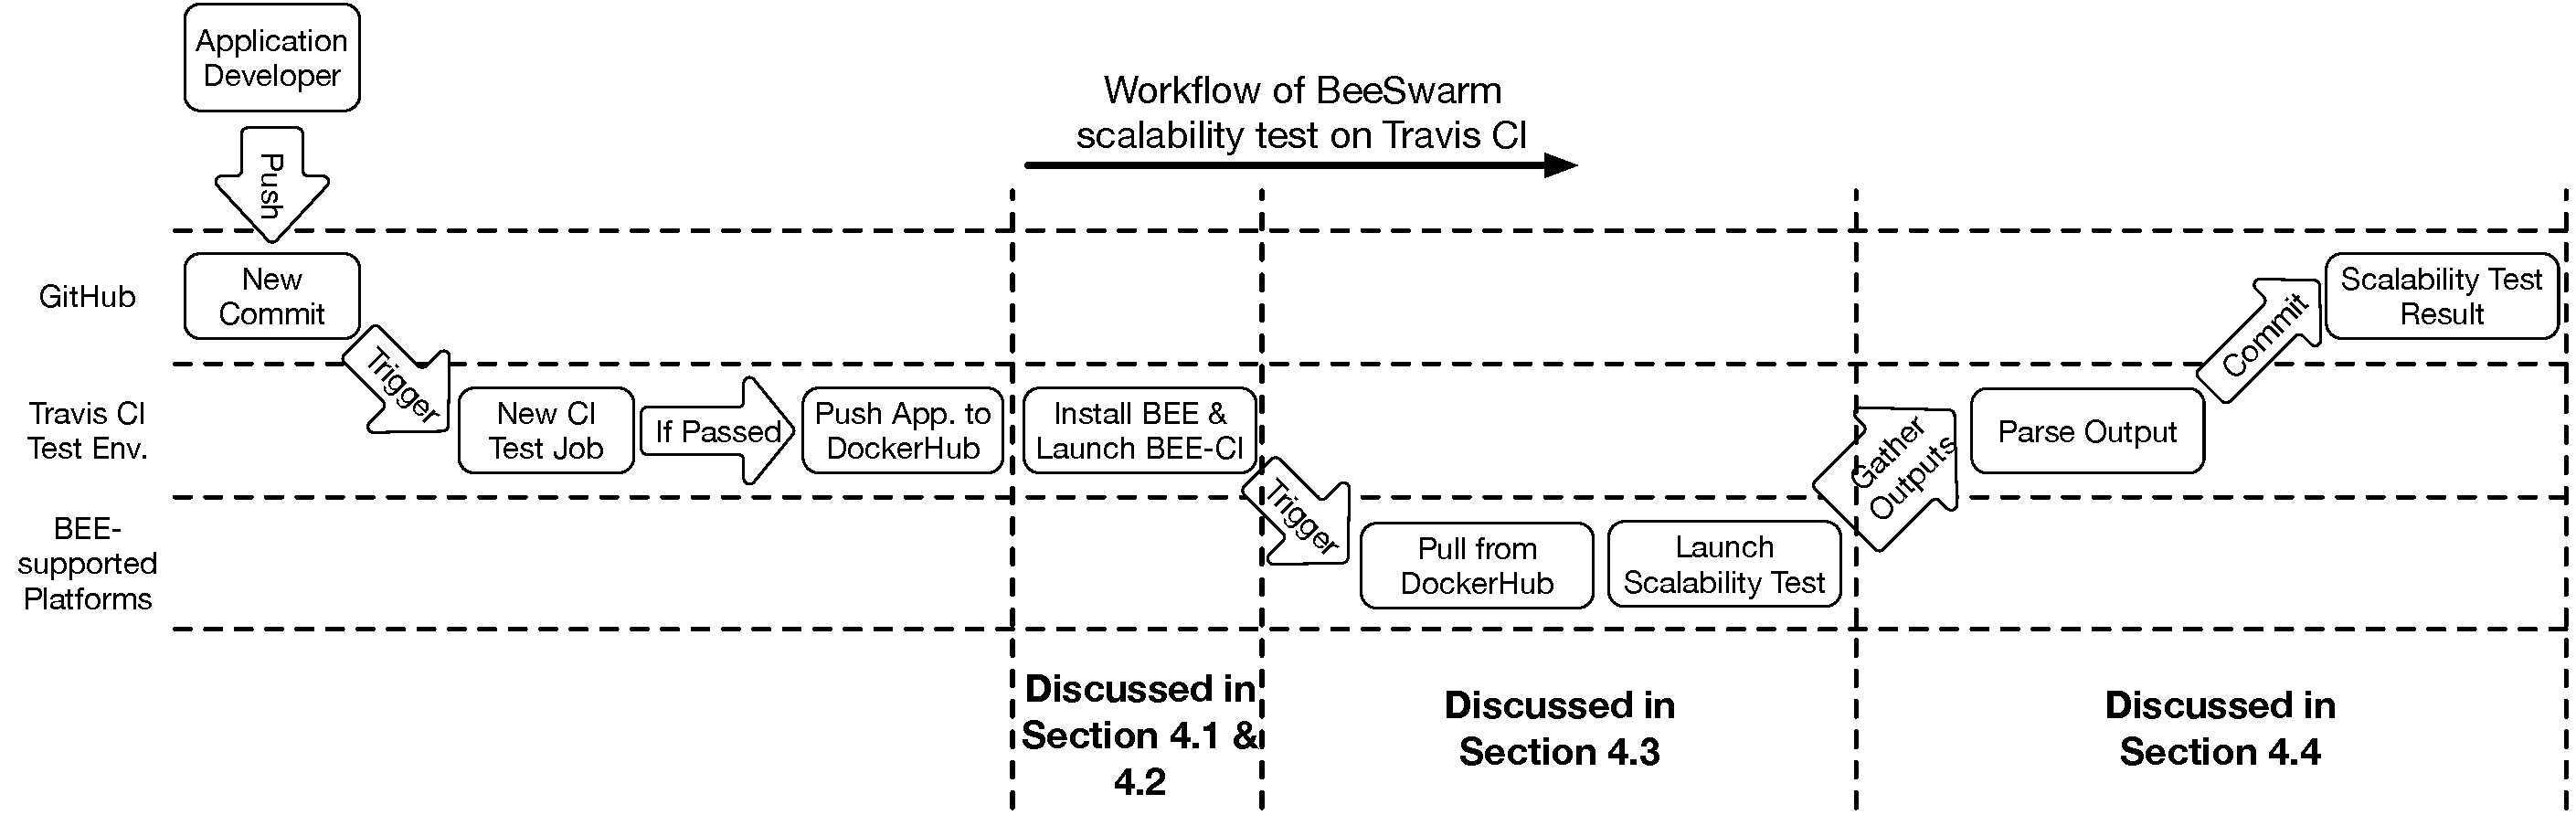
\includegraphics[width=1\textwidth]{figures/CI-workflow.pdf}
    \caption{Overall Workflow of BeeSwarm CI Scalability Test. 
    %\textcolor{red}{Can we add some horizontal lines to partition the steps of workflow to make them mapping 4.1-4.4? And move this graph to page 3, on top of it.}
    }
    \label{overall}
\end{figure*}
\section{Motivation}
\label{motivation}

\begin{table}[h]
\centering
\caption{Several commits in the Legion commit tree that may cause the performance improvement after commit 4400.}
\label{commits}
\begin{tabular}{|p{0.3cm}|p{5.8cm}|}
\hline
\multicolumn{1}{|c|}{Commit HASH} & \multicolumn{1}{c|}{Commit message}                                                                                                  \\ \hline
725e549dc                         & legion: fixing a potential hang with old-style bounds checking                                                                       \\ \hline
3edff3290                         & regent: small bug fix to openmp code generation for regent                                                                           \\ \hline
d0b157755                         & tools: small bug fix for legion prof ascii deserializer                                                                              \\ \hline
1162649ea                         & legion: small bug fix for dependence analysis of close operations involving different children in different modes for the same field \\ \hline
2818b5fe9                         & legion: small bug fix for remote advances of version numbers                                                                         \\ \hline
824d6c77d                         & legion: fixing a bug where we were not properly paging in version states for remote virtual mappings                                 \\ \hline
\end{tabular}
\end{table}

In this section, we use an example to motivate our work by showing necessity of having automatic scalability test in CI. In \textbf{Fig. \ref{exp}} we show the performance of Legion changes as developers make progresses. However,  it is hard to find out the exactly which commit(s) causes the performance change. For example, the performance of Legion improved significantly from commit \texttt{1e96} to \texttt{4400}. Commit \texttt{4400} is a merge operation between two branches, which totally contains about 61300 lines of code changes composing hundreds of commits. It is hard to tell which commit(s) causes the performance improvement. By searching the commit tree of Legion, we found several commits focusing on bug fixing that may potentially affect performance. We list several of them in \textbf{table \ref{commits}}. So, if scalability test was available in the CI for Legion upgrade, we would be able to easily find the root cause of the performance change by searching in the scalability test results for each commit and keep tracking the changes that benefit or hurt the scalability. 

%\textcolor{red}{In this section, go unfold the example of figure 1. First of all, still focusing on the figure 1, pick up 4400 and 1e96 (it also ok if we also want to pick other pair, but this pair is so catching that we cannot miss), explain the changes in statisics (like LOC of changes, see my email). Adding a table with potential impacts to performance gains coming from the commit tree. We don't need to give any judgement but guess. At the end of this section, also point out how difficult it is for code reviewers and developers to figure out the relationship between change-of-code and performance if scalability test is not included in CI.   }


\section{Background}
\label{background}
\subsection{Build and Execution Environments (BEE)}
\texttt{BEE} \cite{bee,beeflow} is a %\trandles{remove 'Docker-based' because BEE can use multiple container runtimes} 
containerization environment that enables HPC applications to run on both HPC and cloud computing platforms. \texttt{BEE} provides a unified user interface for automatic job launching and monitoring. \texttt{BEE} users only need to wrap their applications in a standard Docker image and provide a simple \texttt{BeeFile} (job execution environment description) to run on \texttt{BEE}. Since the same Docker image is used %\trandles{change to "Docker image is used"} 
 across platforms, no source code modification is necessary. %In addition, \texttt{BEE} solves the security constraint of HPC environment that cannot be addressed with current Docker daemon.%\pat{isn't this off I'm not sure most people will think of Docker as secure}
 %\trandles{I agree with Pat. BEE doesn't solve using Docker securely in an HPC environment}
In this work, we build \texttt{BeeSwarm} based on \texttt{BEE}, so it naturally inherits all benefits of \texttt{BEE}. This allows us to build a unified scalability test system across multiple platforms. 



\subsection{Continuous Integration (CI)}
CI was first named and proposed by Grady Booch in 1991. Its aim was to greatly reduce integration problems. CI was initially combined with automated unit testing to run on the developer's local machine before committing to the central code repository.  However, as software being developed becomes more complicated and more people are involved in developing, localized testing becomes inefficient and the code base on each developer's machine can easily become outdated, so integration can still be problematic. The longer a branch of code remains checked out, the greater the risk of multiple integration conflicts and failures when the developer branch is reintegrated into the main line. So, centralized build servers are used for CI. The build servers can perform more frequent (e.g., every commit) test runs and provide reports back to the developers. Driven by these benefits many HPC application development projects are now using CI. For example, almost all projects in Next-Generation Code Project in Los Alamos National Laboratory are using CI \cite{daniel2016lanl}. Currently, many CI tools are available to developers such as Travis CI, Circle CI, Codeship, etc. Many computing platforms also provide CI as a feature in their services such as AWS, Azure, etc. However, current designs of CI services only focus on detecting software bugs in the HPC softwares. To the best of our knowledge, none of the current work can easily enable automatic scalability tests in CI. So, in this work we propose to enable easy scalability tests for HPC developers. %\paul{Is it valuable to reference studies that have sought to analyze the additional value provided via CI or has it been generally accepted that CI is a good thing?} %\pat{it couldn't hurt}

\section{BEE Framework Design}
\texttt{BEE} framework is designed to efficiently organize and manage available computing resources, automatically deploy a Docker-enabled environment, and execute a user's Dockerized application with constant monitoring and scheduling. 

As shown in \textbf{Algorithm \ref{bee}}, we outline the general workflow of \texttt{BEE} framework. First, users need to provide all the computing resources available. This can be HPC systems or cloud computing systems or both with priorities of using these computing resources. For example, when running a compute intensive application, users may want to prioritize systems with higher computing performance. Then, users need to provide a Dockerized application with an input stack and a configuration file.

Before execution, \texttt{BEE} picks the system with the highest priority (\textbf{Line 3}). Then, it deploys the Docker-enabled execution environment on the target system. If the execution target environment is HPC system, \texttt{BEE-VM} is deployed. If the execution target environment is AWS or Chameleon Clound, then \texttt{BEE-AWS} or \texttt{BEE-Chameleon} is applied. Both will be discussed in later sections. After the execution environment is deployed, BEE checks whether the current application is in an initial stage or needs to restore from a previous checkpoint. If it is in an initial stage, \texttt{BEE} attaches the input stack and runs the application as shown in \textbf{Line 8 and 10}. Otherwise, \texttt{BEE} first migrates previous intermediate data checkpoints from the previous system to the current system (\textbf{Line 5}) then attaches the data and restores the checkpoint (\textbf{Line 6}) before running. 

During execution, \texttt{BEE} monitors the current state of the running application. When it is close to the end of the current time slot, \texttt{BEE} checks whether the current application has completed. If so, \texttt{BEE} outputs the result and stops. Otherwise, if the application has a checkpointing procedure and is indicated by the user, \texttt{BEE} initiates the checkpointing procedure and marks $need\_migration$ to ensure the application will resume from the current execution stage for later runs. When finishing the checkpointing procedure, \texttt{BEE} checks for the next available system to run. If no other computing systems are available, \texttt{BEE} saves the checkpoint to disk, until the user indicates new computing resources are available.
	

\begin{algorithm}
\caption{BEE Framework}
\label{bee}
\begin{algorithmic}[1]
\REQUIRE{$HPC/Cloud_1$: [Host node: $H_1$, $H_2$,..., $H_k$][Time slot: $T_1$]}
\REQUIRE{$HPC/Cloud_2$: [Host node: $H_1$, $H_2$,..., $H_k$][Time slot: $T_2$]}

{...}

\REQUIRE{$HPC/Cloud_m$: [Host node: $H_1$, $H_2$,..., $H_k$][Time slot: $T_m$]}
\REQUIRE{Computing resource priority list: $L$}
\REQUIRE{User Dockerized application}
\REQUIRE{Input data: $D$}
\REQUIRE{User defined hardware configuration: uconf}

\STATE $need\_migration \leftarrow$ False
\STATE $lastHost \leftarrow$ N/A

\WHILE{H $\leftarrow$ get\_top($L$)}
	\IF{$need\_migration$ is True}
		\STATE data\_tranfer($lastHost$, $H$, $D$)
		\STATE restore\_data\_checkpoint($D$, $H$) \bluecomment{Load data checkpoint into H}
	\ELSE
		\STATE load\_initial\_data($D$, $H$) \bluecomment{Load initial data into H}
	\ENDIF
	
	\bluecomment{Deploy BEE-VM or BEE-AWS}
	
	\STATE deploy\_bee($H$, $user\_application$, $uconf$)

	\WHILE{$H$ running normal AND Running-time not close to $T$}
		\STATE Monitor($H$)
	\ENDWHILE

	\IF{execution incomplete}
    	\STATE pause($H$)
		\STATE $D \leftarrow$ data\_checkpoint($H$) \bluecomment{Checkpoint application data}
		\STATE $need\_migration \leftarrow$ True
		\STATE $lastHost \leftarrow$ H
		\STATE stop($H$)
	\ELSE
		\STATE stop($H$)
		\STATE result $\leftarrow D $
		\STATE terminate() 
	\ENDIF
\ENDWHILE

\IF{execution incomplete}
		\STATE $D\leftarrow$ data\_checkpoint($H$)
		\STATE stop($H$)
		\STATE store $D$ when no resource available
\ENDIF

\end{algorithmic}
\end{algorithm}


\section{BEE-VM Design}
Linux container technologies (e.g., Docker) enable consistent software and hardware environments for development, build, and deployment. By using Docker, developers only need to build their application once in a Docker container image on their local machine; then, the dockerized application can run on any Docker-enabled machine. However, Docker is not supported on production HPC systems. Existing containerization solutions on current HPC systems typically require customized HPC environments. The lack of a robust and universal solution to containerization in HPC and the requirement of system customization limits the practicality of container deployments across HPC machines.
  
To overcome the constraints and provide a more flexible runtime environment, we designed a backend for \texttt{BEE}, the \texttt{BEE-VM}, which creates a VM layer on top of the host and then deploys Docker on the VM layer; as shown in \textbf{Fig. \ref{bee-framework}}. Besides providing a standard updated Docker capability to HPC system, additionally the VM layer also brings the following advantages: First, with full control over VM, we can create consistent environments for Docker across platforms. As a result, we can deploy \texttt{BEE} on both HPC and AWS with user applications unmodified. Second, Docker containerization ensures the reproducibility across  different software stacks and OSes, while VM guarantees the reproducibility accross different hardware infrastructures, which can be a problem if the container is running directly on the host.  

\begin{figure}[h]
%\vspace*{-1em}
    \centering
    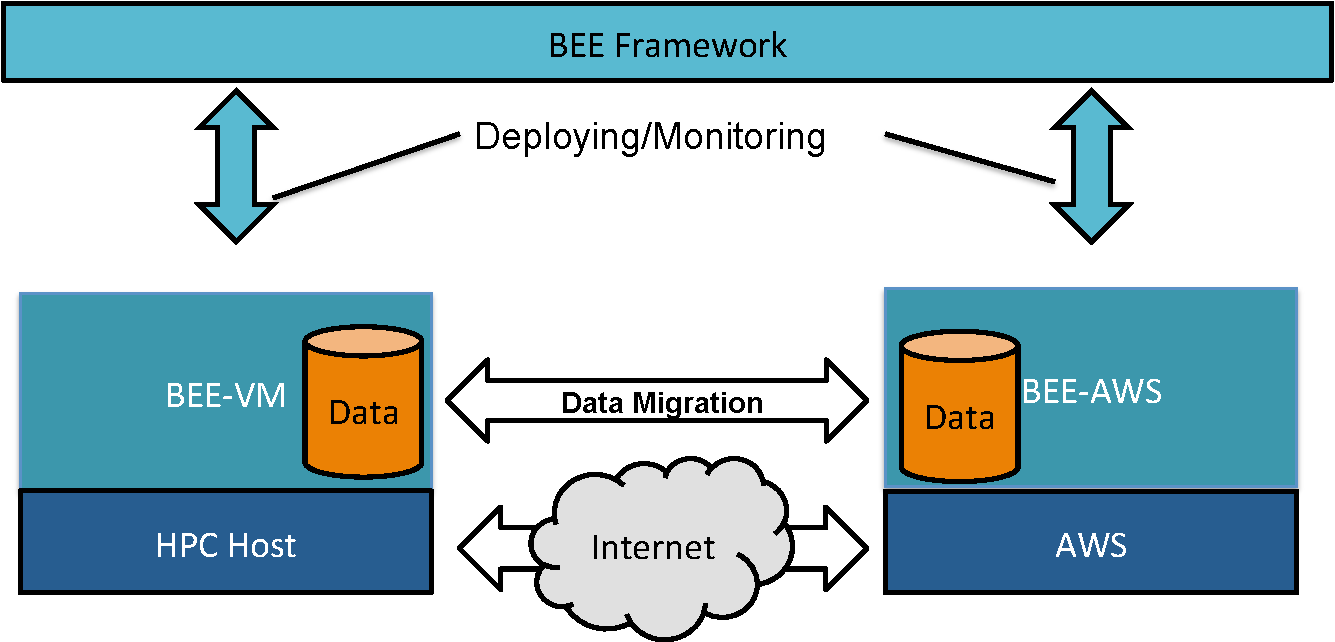
\includegraphics[width=0.35\textwidth]{figures/bee-framework.pdf}
    \caption{BEE Framework}
    \label{bee-framework}
%\vspace*{-1em}
\end{figure}


 The design details of \texttt{BEE-VM} include several parts: network design, storage design, and BEE-VM deployment process. We discuss them in detail in the following sections.
 
\subsection{Network Design}
The network design of \texttt{BEE-VM} mainly targets two functions. First, we need to dynamically configure and deploy our VM and Docker container. This needs to be done automatically and remotely by \texttt{BEE}. We choose to utilize SSH for remote configuration. Also, since we are aiming at HPC application and most HPC applications require MPI, we need to dynamically compose a network for MPI communication between different computing nodes. For enabling that, we create a virtual subnet comprised of all VMs and corresponding Docker containers, so that they can communicate with each other.

\subsubsection{VM layer}
We first discuss the network design at the VM layer. This is necessary because the Docker container will rely on the VM's network configuration for network in the container. 

In order to enable the SSH connection to the VM through the host, the hypervisor is configured to use port forwarding to map an unused port on the host to the SSH port on the VM. However, this makes the virtual network interface card (vNIC) hard to utilize by MPI. Although some MPI libraries can be configured to use a designated port and can cooperate with port forwarding, many commonly used MPI libraries (e.g., OpenMPI) use random ports, which is not easy to work with the port forwarding mechanism. So, we created a second vNIC dedicated for MPI communication. 

However, allowing application in different node communication to each other through the second vNIC is challenging. The main challenges of designing the network for VMs is that the root privileges are not assigned to regular user but most of the suitable VM networking configurations do require root privileges (e.g., bridging network). To address this limitation, we designed two user space solutions for connecting all second vNICs on HPC systems.



\begin{comment}
\textbf{Solution 1: 2 NICs}
We design our first solution on the `Galton` nodes of our testbed cluster machine. Each `Galton` node has two physical NICs. So, we use the port forwarding combining the SSH virtual NIC with one physical NIC and use simple pass-through mode to combine the MPI virtual NIC with the other physical NIC. This is the simplest design in our two solutions. However, this solution is limited to deployment on computing nodes with multiple physical NICs. 

\begin{figure}[h]
    \centering
    \caption{Network Design using two NICs}
    \label{2nic}
    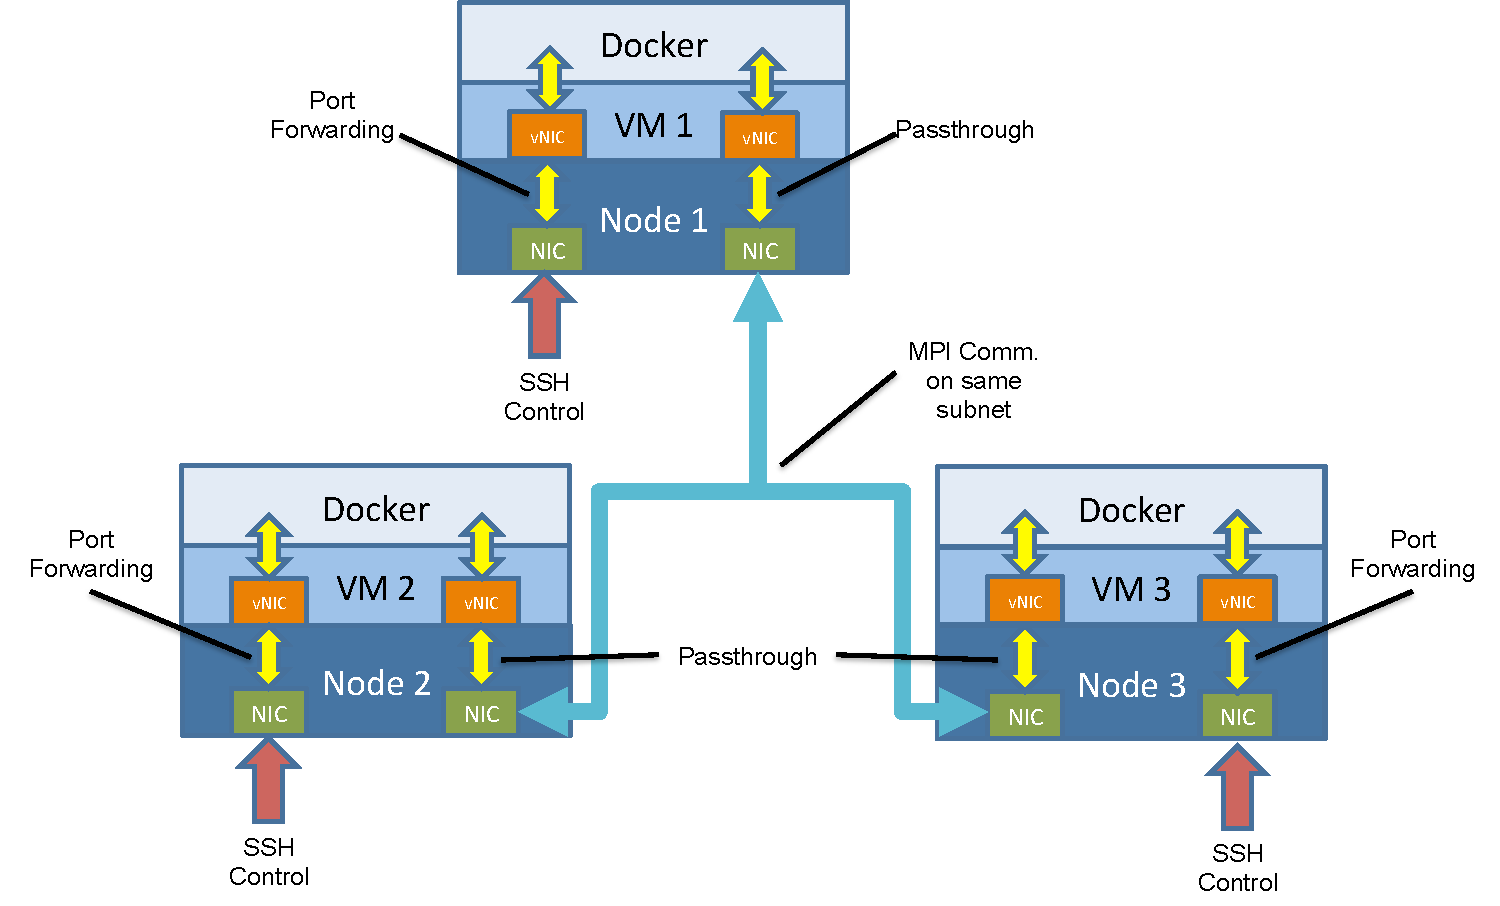
\includegraphics[width=0.5\textwidth]{figures/2nic.pdf}
\end{figure}

\end{comment}
 
\textbf{Network Solution 1: Multi-cast}
In the first solution, we use multi-cast subnet to connect all second vNICs of all VMs together for MPI communication. Since all vNICs are connected to the same subnet, there is no restriction on port usage, so any MPI library can be used. The advantage of this design is that the configuration is simple, and if one node in the multi-cast network failed, it will not affect the connection in between other nodes, which can easily cooperate with a potential fault tolerance mechanism. This network design works best on applications with intensive all-to-all or one-to-all communications, since all packages are naturally sent to all nodes. However, if one-to-one communication is more frequent, the multi-cast network brings high communication overhead, since it generates more data packages in the subnet than necessary. 

\begin{figure}[h]
	%\vspace*{-1em}
    \centering
    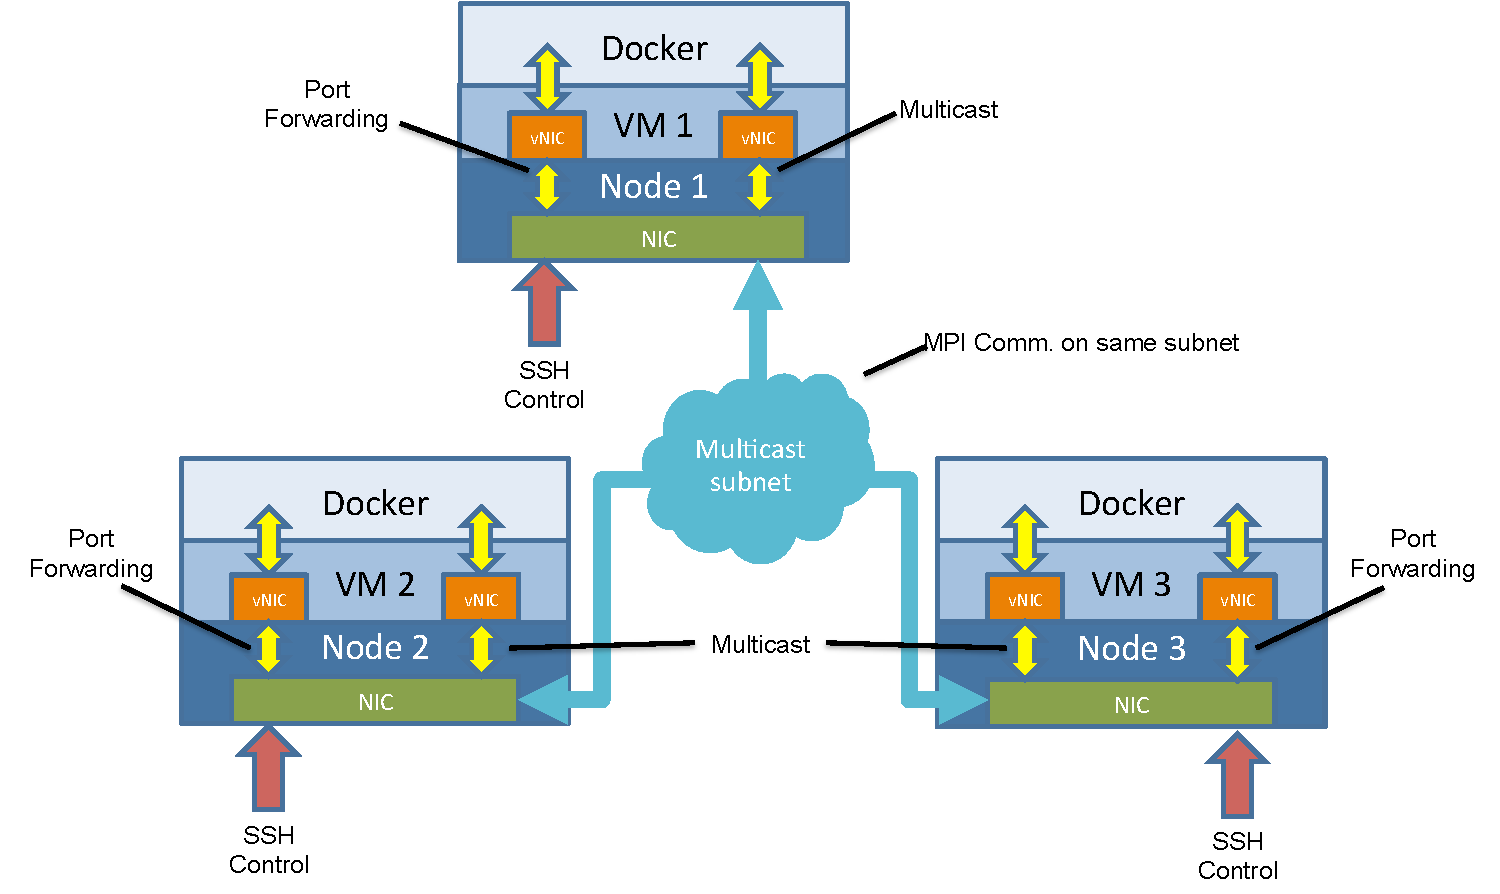
\includegraphics[width=0.5\textwidth]{figures/mcast.pdf}
    \caption{Network Design using Multi-cast}
    \label{mcast}
    %\vspace*{-1em}
\end{figure}

 
\textbf{Network Solution 2: P2P sockets}
In our second solution, we connect each second vNIC from each VM using point-to-point (P2P) socket connection. This is similar to the wired Ethernet connection between computing nodes in HPC system, except instead of relying on a physical switch we map out a specific routing topology. Since there is a P2P routing path between nodes, there are no unnecessary data packages in the network. However, socket connections between nodes may route via intermediate nodes, so if one node fails, it may break several connected nodes, complicating any potential fault tolerance mechanisms. Also, the performance of this kind of network is affected by the connection pattern between nodes, so we adopt two connection patterns in this solution (more patterns will be studied in the future).

\begin{figure}[h]
  	%\vspace*{-1em}
    \centering
    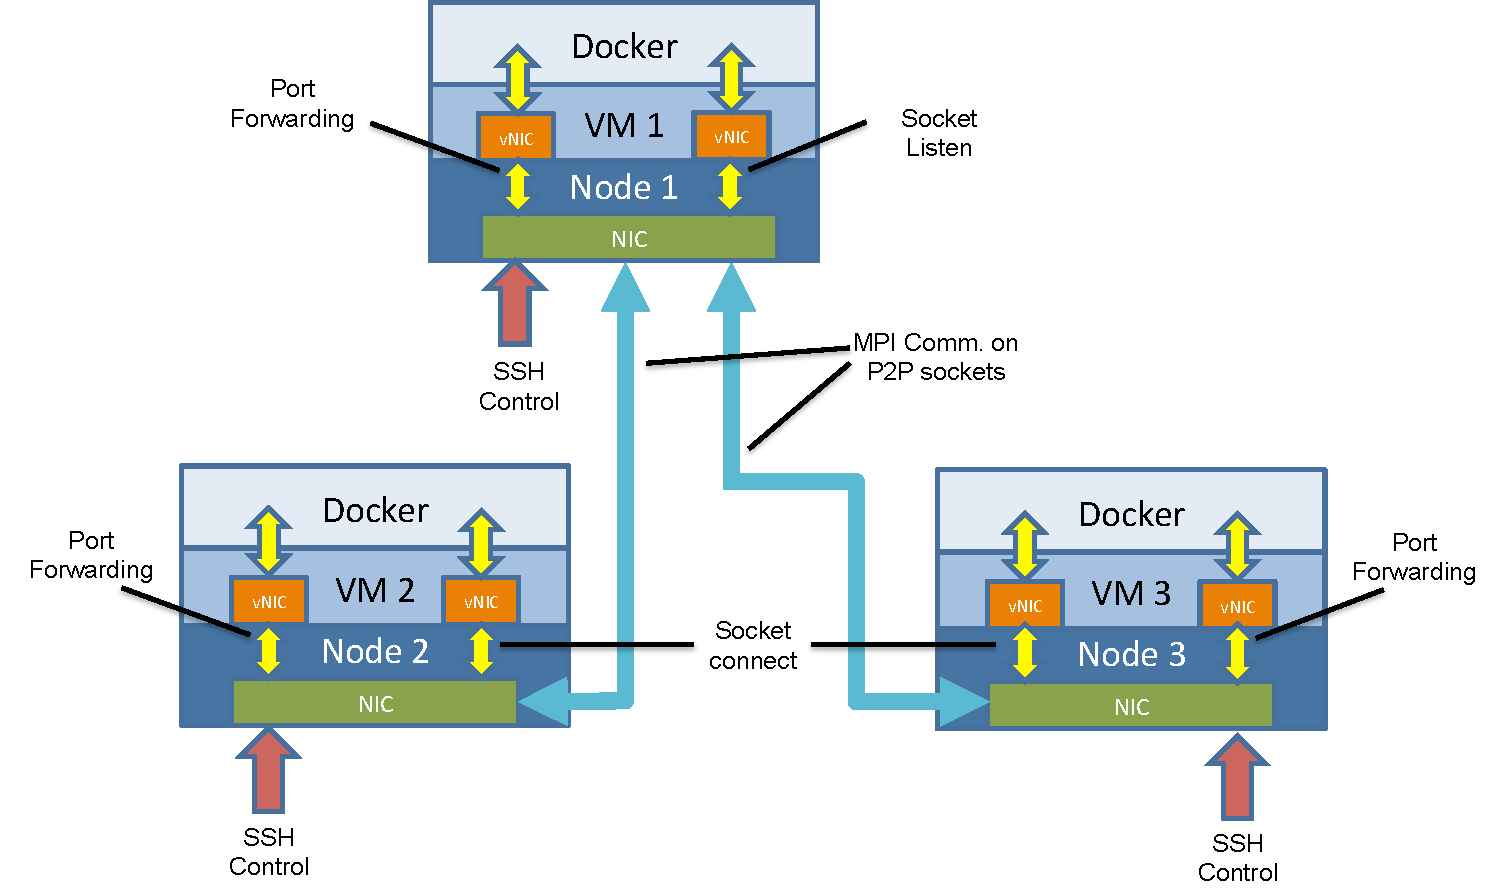
\includegraphics[width=0.5\textwidth]{figures/p2p.pdf}
    \caption{Network Design using P2P sockets}
    \label{p2p}
    %\vspace*{-1em}
\end{figure}

\begin{itemize}
\item \textbf{Star-shaped connection}
In the first approach, we connect nodes using star-shaped topology with the master node in the center. This connection pattern can effectively minimize connection hops between each pair of nodes ($O(1)$). However, since all communication must go through the center node, it may become a hot stop in the network, especially for applications involve intensive network communication or the shared storage design that requires network communication.
\item \textbf{Tree-shaped connection}
The second way to connect all nodes is using tree-shaped topology with the master node as the tree root. In this design, we use a binary tree structure. This connection can mitigate the hot spot issue, but it also increases connection hops between each pair of nodes ($O(n\log{n})$). 
\end{itemize}

\subsubsection{Docker container layer}
Based on the network of VM layer, we design the network between Docker containers. There are several network configurations for the Docker containers; however, to minimize network overhead, the most direct configuration is network pass-through. Essentially, all network interfaces on the VM are exposed to the Docker container. Since there is no additional buffer or translation in between, it brings the least overhead. However, it is also considered as the least secure configuration, since everything is exposed. But since we deploy the Docker inside VM, this extra layer already provides enough isolation, so there is no extra security issue here. Since the presented network interfaces are exactly the same between the VM and the Docker container inside it, the software level configuration (e.g., SSH, MPI, etc.) is exactly the same.

\subsection{Storage Design}
\subsubsection{VM layer}
In this section, we discuss the design of shared storage system of \texttt{BEE-VM}. General HPC applications usually use some kind of shared file system (e.g., NFS) to share data between processes in real-time. To provide the same environment, we need to build a shared file system across different nodes in \texttt{BEE-VM}. To enable light-weight cross-platform migration, we aim to separate data from the virtualized operating system itself. This separation allows users to easily migrate their data to another platform without transferring heavy operating system files. We design two architectures to allow different processes in different nodes to share files in real-time.

\textbf{Storage Solution 1: Extra Data Image + NFS}
In our first solution, we build an extra data image and mount it as the second disk. Due to the copy-on-write characteristic of most virtual images, files updated by one machine are not visible by other machines in real-time. So, we choose to mount this data image only to the master node, and use NFS to share this mounted data disk with other VMs. By using the extra data image, data can be easily migrated.  Before computation, input data can be first loaded into the image offline. After execution, the output data is also stored in this image. To move the data to other parts of the user workflow, the user only needs to unmount the data image from the master node of the current \texttt{BEE} cluster and mount it to the master node used for the next stage computation. Also, the image encapsulation can protect data integrity. However, the data image is shared with other worker nodes via NFS, which highly depends on the performance of the virtual network. If the user's application is storage I/O intensive and the network bandwidth is limited, it may consume too much of the network resource, which may degrade MPI communication performance.


\begin{figure}[h]
	%\vspace*{-1em}
    \centering
    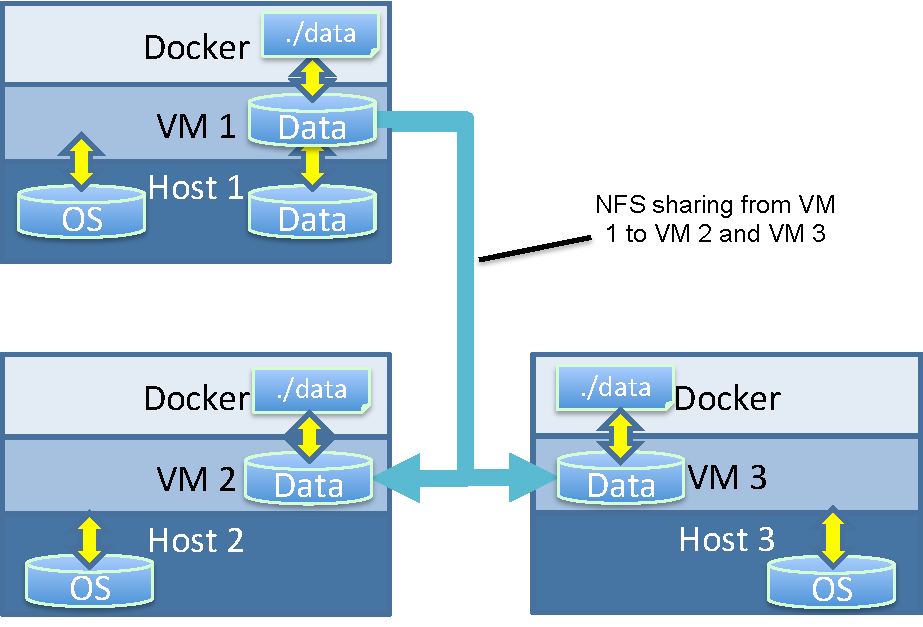
\includegraphics[width=0.5\textwidth]{figures/fs1.pdf}
    \caption{Shared Storage Design using Extra Data Image + NFS}
    \label{fs1}
\end{figure}


\begin{comment}
\subsubsection{Only NFS}
In our second solution, we aim to reduce the dependency on a virtual shared filesystem. Instead of building our own NFS sharing environment, we mount the NFS standard filesystem that is commonly used on most HPC systems. Each VM explicitly mounts the same path within the shared filesystem. Data in the same directory is shared between different host nodes via  existing fast dedicated shared hardware resources. Since a host directory is mounted, the data is also accessible from the host during execution, which can be useful for output monitoring or sampling for in-situ analysis. This is not possible if we use the first solution, since data is not readily accessible outside the data image. This solution only relies on the network between host and VM, which saves most virtual network bandwidth for MPI communication.


\begin{figure}[h]
    \centering
    \caption{Shared Storage Design using Only NFS}
    \label{fs2}
    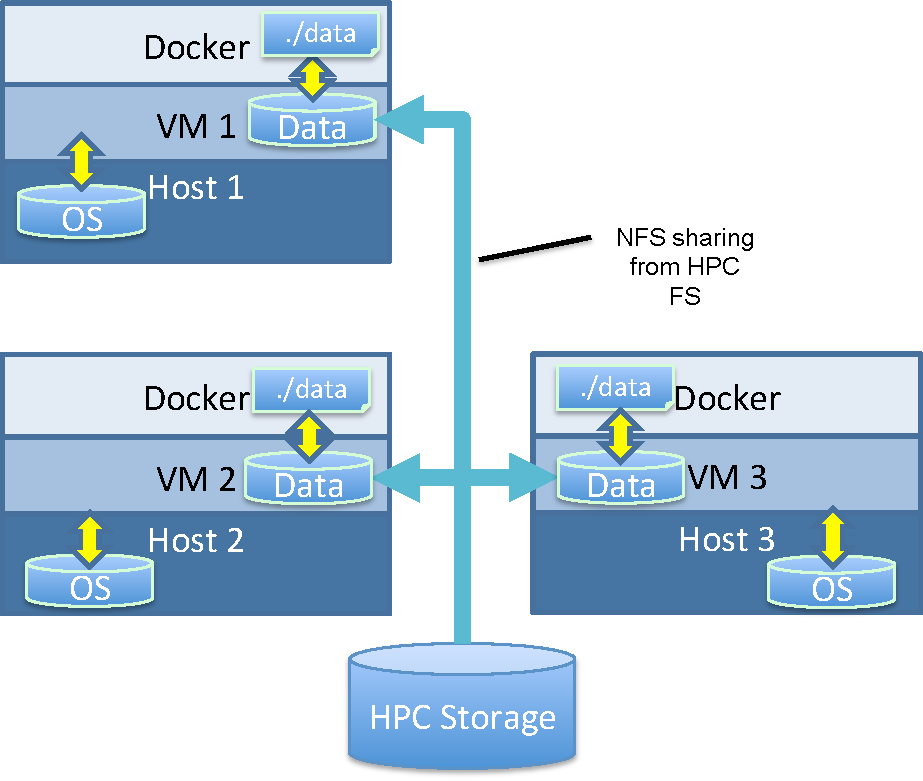
\includegraphics[width=0.4\textwidth]{figures/fs2.pdf}
\end{figure}
\end{comment}

\textbf{Storage Solution 2: Virtio}
In our second solution, we eliminate all the dependency on the virtual network. We use the Virtio feature \cite{russell2008virtio} in QEMU to map a host directory to a directory in VMs. It only requires minimum configuration at VM boot time. Each machine maps the same directory, so the data is shared using file-sharing capability that is commonly used in most HPC systems (e.g., NFS, Lustre, etc.), and it is also visible to the host in real-time. Since it does not rely on the virtual network, the whole virtual network is saved for MPI.

\begin{figure}[h]
	%\vspace*{-1em}
    \centering
    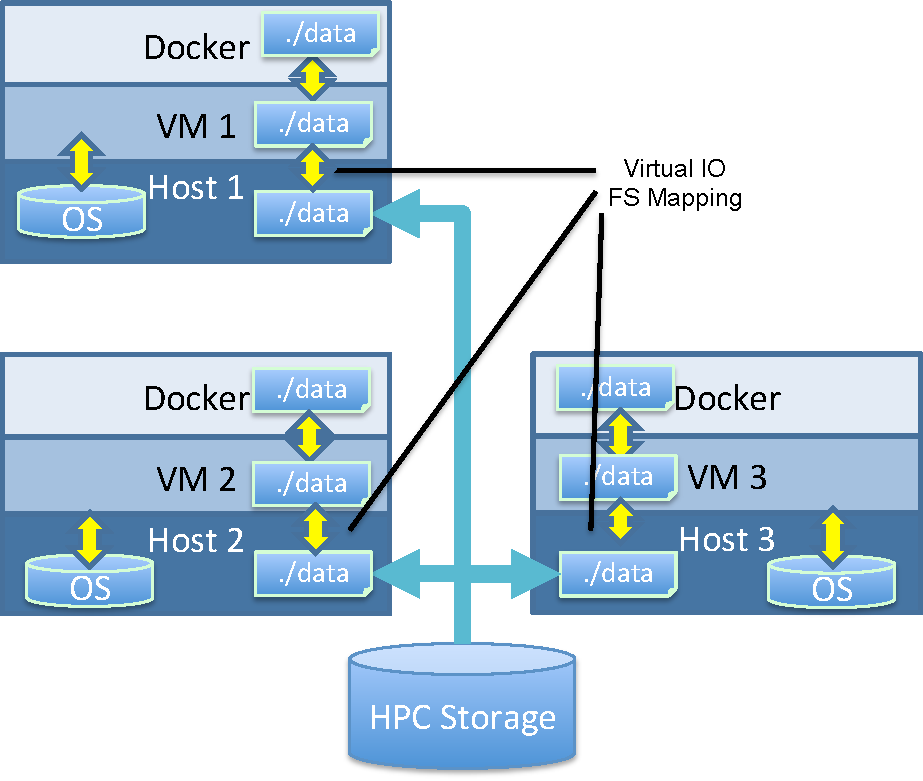
\includegraphics[width=0.5\textwidth]{figures/fs3.pdf}
    \caption{Shared Storage Design using Virtual IO}
    \label{fs3}
    %\vspace*{-1em}
\end{figure}

\subsubsection{Docker container layer}
Finally, for data sharing in the Docker layer, we use the data volume mount feature in Docker to mount the shared folder in the VM to a directory in Docker. Since Docker runs as a process at the VM layer, mounting the data volume adds negligible overhead. This configuration is also compatible with all data-shared mechanisms in the VM layer.

%\begin{comment}
\subsection{BEE-VM Builder}
VM plays an important role in \texttt{BEE-VM}. The VM is the core of \texttt{BEE-VM} that brings computing resources from host, virtual network, shared storage, user provided Dockerized application and Docker container management together. The VM in \texttt{BEE-VM} first need to be build and customized by \texttt{BEE-VM Builder} before it can be used. There are two phases in the building process:

\subsubsection{Phase 1}
The first stage in building the VM images for  \texttt{BEE-VM}. This step is done off-line before it is deployed on targeting HPC system. For uniform standard image building process, we designed our \texttt{BEE-VM Image Builder} using Packer \cite{packer}. Packer allows us to build customized images automatically. We can also run our own configure scripts in the VM image to enable more flexible customization. Although it is also possible to configure and customize VM OS in phase 2 after booting VMs, the static customization and configuration of images off-line can save a lot of time. For example, building and installing packages. We aim to minimize on-line configuration as much as possible to reduce \texttt{BEE-VM} deployment time and put most of the customization into the \texttt{BEE-VM Image Builder}. The main customization responsibilities of \texttt{BEE-VM Image Builder} include:
\begin{enumerate}
\item \textbf{Create and configure user accounts:} We need to create a user for the host to login or control the VM.
\item \textbf{Configure network interfaces:} Network interface must be configured in advance before \texttt{BEE} can configure and control the VM after it has started. However many network configurations cannot be determined until boot time, so we design a customize script built in to the image, so that network interface can be customized automatically when the VM started.
\item \textbf{Configure SSH server/client:} SSH is required for \texttt{BEE} to control VM and it is also important for MPI. So, we need to configure SSH key pairs and customized port numbers in this step.
\item \textbf{Install essential packages and tools:} Many packages and tools are required including MPI and Docker.
\item \textbf{Configure proxy settings:} Most institutional HPC system requires some kind of proxy setting in order to connect to the Internet. 
\item \textbf{Configure shared storage:} We need to pre-configure the VM image for mounting shared storage system. For example, configuring NFS server.
\end{enumerate} 

\subsubsection{Phase 2}
This phase is done when deploying \texttt{BEE-VM} on target HPC system. The base image created from phase 1 is highly reusable. Each \texttt{BEE-VM} uses the base image to create a dedicated image for the current \texttt{BEE-VM}. When \texttt{BEE-VM} started, user's Dockerized application is placed in it. This can be done in several ways. User can provide Docker image from public or private DockerHub or build Docker image from Dockerfile. After than, the building process of \texttt{BEE-VM} is done.

%\end{comment}

\subsection{BEE-VM Deployment}
\textbf{Algorithm \ref{bee-launch}} shows the workflow in \texttt{BEE} used for launching \texttt{BEE} cluster on a given platform. Although the specific process varies from HPC system to cloud computing system, the general procedures are the same. At first, the launcher needs to know how many and which nodes are available. Then, the user Dockerized application is provided, which can be in either Docker image form or Dockerfile form. Finally, a user-defined hardware configuration file may also be provided, which is used when starting VMs. 

There are four stages for launching HPC applications in \texttt{BEE}. In the first stage, a new \texttt{BEE} cluster is initialized with optional given name. This stage registers each available host to the virtual cluster. Second, \texttt{BEE-VM} deploys the VM layer. It creates one VM for each host, and then configures and assigns the VM to the  host. In \textbf{line 13}, \texttt{BEE-VM} starts a VM in parallel using MPI. In the third stage, \texttt{BEE-VM} starts to deploy the Docker layer. Depending on what the user provides, \texttt{BEE-VM} will either pull the Docker image from public/private registries or build a new Docker image from a Dockerfile loaded into the local VM. Finally, in the forth stage, \texttt{BEE} starts the application by launching from the first node (i.e., master node).


\begin{algorithm}
\caption{Deploying BEE cluster on HPC/cloud}
\label{bee-launch}
\begin{algorithmic}[1]
\REQUIRE{Allocated host nodes: $H_1$, $H_2$,..., $H_k$}
\REQUIRE{User Dockerized application (Docker image/Dockerfile)}
\REQUIRE{BEE cluster name: cname}
\REQUIRE{User defined hardware configuration: uconf}
%\STATE \textbf{[Create a new \texttt{BEE} cluster]}

\bluecomment{Create a new \texttt{BEE} cluster}
\STATE $BCluster \leftarrow$ create\_bee\_cluster(cname)
\FOR{$j=1$ to $k$}
	\STATE $BCluster$.register\_host($H_j$)
\ENDFOR
%\STATE \textbf{[Deploy VM layer]}

\bluecomment{Deploy VM layer}
\FOR{$j=1$ to $k$}
	\STATE $vm_j$ $\leftarrow$ create\_vm()
	\STATE $vm_j$.create\_img() \bluecomment{Create image for each VM}
	\STATE $vm_j$.configure(uconf) 
	\STATE $vm_j$.setup\_shared\_vol()
	\STATE $vm_j$.setup\_network()
	\STATE $H_j$.register\_vm($vm_j$)
\ENDFOR
\STATE $BCluster$.mpi\_start\_vms()
%\STATE \textbf{[Deploy Docker layer]}

\bluecomment{Deploy Docker layer}
\FOR{$j=1$ to $k$}
	\STATE $dkr_j$ $\leftarrow$ create\_doocker()
	\IF{user provides Docker image}
		\STATE $dkr_j$.img\_pull(d\_img)
	\ELSE
		\STATE $dkr_j$.img\_build(d\_file)
    \ENDIF
	$vm_j$.register\_docker($dkr_j$)
\ENDFOR
\STATE $BCluster$.mpi\_start\_dockers()
\STATE \textbf{[Start user application]}
\STATE $BCluster$.$vm_i$.$dkr_1$.start()

\end{algorithmic}
\end{algorithm}

\begin{comment}
\subsection{BEE-VM Object-oriented Design}

\begin{figure}[h]
\vspace*{-1em}
    \centering
    \caption{BEE Object-Oriented Design}
    \label{ood}
    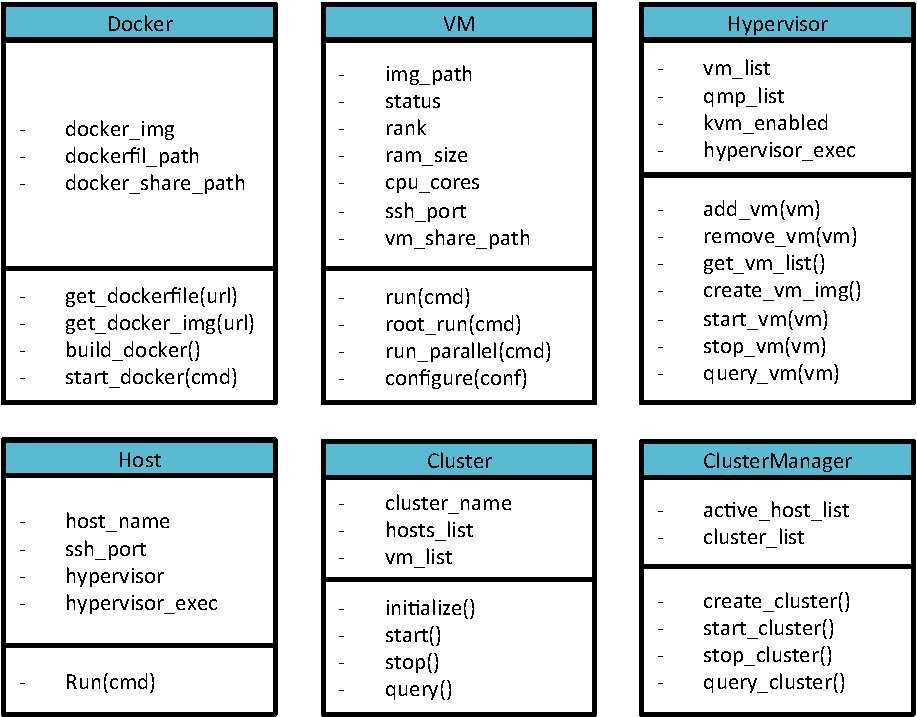
\includegraphics[width=0.5\textwidth]{figures/ood.pdf}
    \vspace*{-1em}
\end{figure}
In this section, we discuss the design details of our \texttt{BEE} framework. To better manage large scale \texttt{BEE} clusters and for extensibility consideration, we choose to use object-oriented design in python for \texttt{BEE} as shown in \textbf{Figure \ref{ood}}. We design several key classes for key components in \texttt{BEE} and \texttt{BEE-VM}, including: \texttt{Docker}, \texttt{VM}, \texttt{Hypervisor}, \texttt{Host}, \texttt{Cluster}, and \texttt{ClusterManager}. \texttt{Docker} class stores Docker-related information. For example, Docker image name, Dockerfile path, Docker's running state and the directory in Docker that is shared between containers. It also contains necessary functions to control or run commands in the Docker containers. \texttt{VM} class stores VM-related information, including the VM instance, current hardware configurations, network settings, VM image file path, shared storage directory, etc. It also has necessary functions to control the VM. However, we leave start/stop/query function to the \texttt{Hypervisor} class, since implementation of those functions are hypervisor-specific. \texttt{Hypervisor} class stores hypervisor-related information. For example, the path to the hypervisor binary, KVM availability, and a list of VMs that it are currently running. Since we allow different machine to use different hypervisors, we inherit the \texttt{Hypervisor} class to get the hypervisor class for specific hypervisors. For example, we have a \texttt{QEMU} class that is targeting for QEMU hypervisor. Besides all the functions inherited from \texttt{Hypervisor} class, it also has some QEMU-specific functions, like QMP VM monitor functions. \texttt{Host} class maintains all the information of each host, including the host name, username, port number and the hypervisor that is currently running on it. It also has functions used to execute commands on the host. \texttt{Cluster} class maintains the information of a virtual \texttt{BEE} cluster, including cluster name, all host nodes and the VMs involved, network configuration for this cluster, etc. It also has functions to control and query the cluster. \texttt{ClusterManager} class is used to manage multiple clusters on a computing system. It maintains all the active host nodes on the current system, so that they can be shared between clusters. It provides necessary functions to control each clusters. 
\end{comment}
\section{BEE-AWS Design}
AWS is a highly usable computing environment for cloud and HPC users. To provide a similar Docker-enabled environment on AWS, we designed another back-end \texttt{BEE}, the \texttt{BEE-AWS}. It enables the user to run their Dockerized application on AWS using \texttt{BEE-AWS} the same way as they run on the HPC system using \texttt{BEE-VM}. Since both the storage and network on AWS are highly optimized and their configurations are hidden from users, the design of \texttt{BEE-AWS} is relatively simpler than \texttt{BEE-VM}. In \texttt{BEE-AWS}, it first launches an AWS instance based cluster using BOTO API \cite{BOTOAPI} with optimized network configuration and a shared EFS storage. Then, it loads the user application's input data into EFS for storage sharing. Next, \texttt{BEE-AWS} controls each instance to obtain Docker images either from public/private docker registries or builds Docker images from Dockerfiles. Finally, it starts the user application in Docker containers.
\section{BEE-Chameleon}
Chameleon Cloud \cite{chameleon} is a highly configurable experimental environment for large-scale HPC and cloud research. We also designed a \texttt{BEE} backend, \texttt{BEE-Chameleon}, for delivering same Docker-enabled environment on Chameleon Cloud. So, BEE users can also run their Dockerized application on Chameleon Could without modification. Chameleon Cloud is managed by OpenStack, which allows us to launch, configure, and control instances on Chameleon Cloud through remote APIs. Chameleon Cloud enables user to have root privileges on their bare-metal machines, so we deploy the Docker layer directly on the host without the VM layer in between. Taking advantage of the Infiniband support in SR-IOV enabled instances, we also enable Infiniband support in \texttt{BEE} through a customized Infiniband-enabled \texttt{BEE} Docker base image. So, users of \texttt{BEE} can have an option to utilize accelerated network in \texttt{BEE-Chameleon} by rebuilding their Dockerized application with our new Infiniband-supported base image.
\section{Experiments}
\label{experiments}
In this section, we conduct experiments to show the performance and scalability of \texttt{BeeSwarm}. We use a Department of Energy (DOE) code, Flecsale \cite{charest2017flexible}, as an example software development project. We deploy \texttt{BeeSwarm} on Travis CI test environment and use Chameleon Cloud \cite{mambretti2015next} as the computation back-end for the scalability tests. The Chameleon Cloud is an OpenStack-based cloud computing platform that offer bare-metal access to all computing nodes. It is currently deployed at University of Chicago and the Texas Advanced Computing Center with total 650 multi-core nodes. We conduct our test on the nodes located at University of Chicago. 

\subsection{Modified Travis CI script}
In this section, we show a sample modified Travis CI script for Flecsale that has \texttt{BeeSwarm} scalability test enabled (\textbf{Listing 1}). Line 1 - 12 are the original Flecsale test code on Travis CI. To enable \texttt{BeeSwarm} scalability test, we only need to add less than 10 lines of simple code (line 13 - 18). The original CI script include building a Docker image  (line 9), running the Docker image (line 10) to correctness test scrips, and push the image to DockerHub if the test was successful (line 12). We add the \texttt{BeeSwarm} configuration and launching scripts after the image is successfully pushed onto the DockerHub. We obtain and install \texttt{BeeSwarm} in line 13 and 14. We add necessary environment variables (for OpenStack and \texttt{BeeSwarm}) in line 15. The scalability test is launched using a simple command in line 16. We add a 120 minutes timeout here since Travis CI would kill a job if a command runs more than 10 minutes by default and a scalability test usually needs more time than that. The actual timeout length can be set based on need of a specific application. Finally, we run the output parser in line 17 followed by pushing scalability test result to original code repository in line 18. It can be seem that with minimum modification current CI scripts can easily enable scalability test through \texttt{BeeSwarm} and the scalability test code is highly portable across any kind of CI service platforms.

\lstset{numbers=left,
xleftmargin=1.5em,
frame=single,
framexleftmargin=2em}


\lstset{language=Java}
\begin{lstlisting}[escapechar=!,
				   caption= Example Travis CI script (\texttt{.travis.yml}) for Flecsale with \texttt{BeeSwarn} scalability test. Highlighted part shows that only simple modifications are required to enable autonomic scalability test.]
language: cpp
sudo: required
services:
 - docker
before_install:
 - git fetch --unshallow 
 - git fetch --tags
script:
 - docker build -t <img> <dockerfile> 
 - docker run <img> <correctness_test>
after_success:
 - docker push <img>
 - !\hl{git clone https://github.com/lanl/BEE.git \&\& cd ./BEE}!
 - !\hl{./install\_on\_travis.sh}!
 - !\hl{source openrc.sh}!
 - !\hl{travis\_wait 120 bee\_ci\_launcher.py -l flecsale}!
 - !\hl{output\_parser.py}!
 - !\hl{push\_results\_to\_repo.sh}!
\end{lstlisting}

\begin{comment}

\end{}
\begin{lstlisting}[language=yaml]
language: cpp
sudo: required
services:
- docker
env:
  matrix:
    - DISTRO=ubuntu_mpi BUILD_TYPE=Debug DOCKERHUB=true
before_install:
 - git fetch --unshallow && git fetch --tags
script:
  - if [[ ${CC} != gcc ]]; then TAG="_${CC}"; fi
  - if [[ ${TRAVIS_BRANCH} != stable ]]; then TAG="${TAG}_master"; fi
  - cp -vr docker ${HOME}/docker
  - sed -i "1s/fedora_serial/${DISTRO}${TAG}/" ${HOME}/docker/Dockerfile
  - cd ../../
  - cp -r ${TRAVIS_REPO_SLUG} $HOME/docker
  - docker build --build-arg BUILD_TYPE=${BUILD_TYPE} 
     --build-arg CC=${CC} 
     --build-arg CXX=${CXX}
     --build-arg CI=${CI}
     --build-arg TRAVIS=${TRAVIS} 
     --build-arg TRAVIS_OS_NAME=${DISTRO}
     --build-arg TRAVIS_BRANCH=${TRAVIS_BRANCH} 
     --build-arg TRAVIS_JOB_NUMBER=${TRAVIS_JOB_NUMBER}
     --build-arg TRAVIS_PULL_REQUEST=${TRAVIS_PULL_REQUEST} 
     --build-arg TRAVIS_JOB_ID=${TRAVIS_JOB_ID}
     --build-arg TRAVIS_TAG=${TRAVIS_TAG} 
     --build-arg TRAVIS_REPO_SLUG=${TRAVIS_REPO_SLUG}
     --build-arg TRAVIS_COMMIT=${TRAVIS_COMMIT}
     -t ${TRAVIS_REPO_SLUG}:${DISTRO}${TAG} ${HOME}/docker/ 
   - docker run -d ${TRAVIS_REPO_SLUG}:${DISTRO}${TAG} /bin/bash
after_success:
   - if [[ ${DOCKERHUB} = true && ${DOCKER_USERNAME} && ${DOCKER_PASSWORD} && ${TRAVIS_PULL_REQUEST} == false && ${TRAVIS_BRANCH} == master && ${CC} = gcc ]]; then
      docker login -u="$DOCKER_USERNAME" -p="$DOCKER_PASSWORD";
      docker push "${TRAVIS_REPO_SLUG}:${DISTRO}${TAG}";
      cd ${HOME}
      git clone https://${GH_TOKEN}@github.com/lanl/BEE_Private.git && cd ./BEE_Private
      ./install_on_travis.sh
      source ${HOME}/build/${TRAVIS_REPO_SLUG}/bee_scalability_test/CH-819321-openrc.sh
      export PATH=$(pwd)/bee-launcher:$PATH
      export PATH=$(pwd)/travis_ci:$PATH
      export PATH=${HOME}/build/${TRAVIS_REPO_SLUG}/bee_scalability_test:$PATH
      cd ${HOME}/build/${TRAVIS_REPO_SLUG}/bee_scalability_test
      travis_wait 120 bee_ci_launcher.py -l flecsale -r $OS_RESERVATION_ID
      output_parser.py
      push_results_to_repo.sh
    fi
compiler:
  - gcc
\end{lstlisting}
\end{comment}

\subsection{Performance of \texttt{BeeSwarm}}
\begin{comment}


\begin{figure}[h]
    \centering
    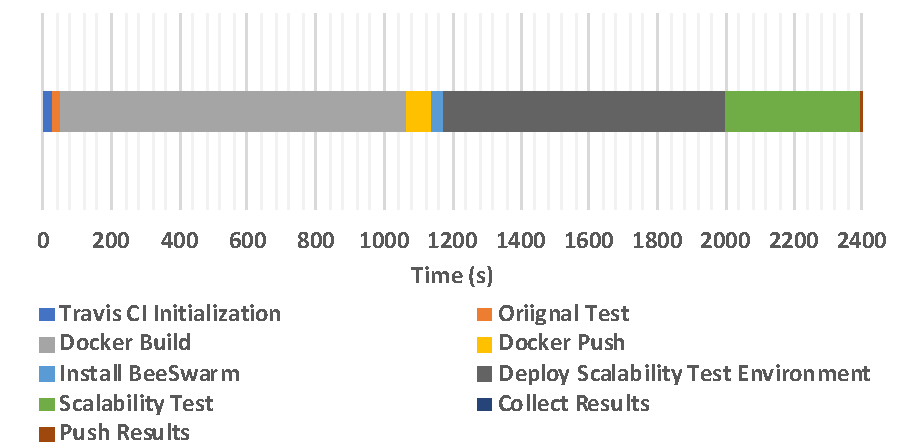
\includegraphics[width=0.5\textwidth]{figures/perf.pdf}
    \caption{Time breakdown of CI for Flecsale with \texttt{BeeSwarm} Scalability Test}
    \label{perf}
\end{figure}
\end{comment}
In order to evaluate the performance of \texttt{BeeSwarm}, we discuss the overhead of launching \texttt{BeeSwarm} and the scalability of \texttt{BeeSwarm} for large-scaled test.

\subsubsection{Overhead of \texttt{BeeSwarm}}
\textbf{Fig. \ref{breakdown}} shows the time breakdown of CI for Flecsale with \texttt{BeeSwarm} scalability test including the original correctness test on Travis CI and one set of multi-node scalability tests using texttt{BeeSwarm}. The scalability test involves different execution configurations that range from 1 process to 128 processes. We can see the major overhead of \texttt{BeeSwarm} comes from deploying the scalability test environment. This is mainly caused by long instance launching time on Chameleon cloud. However, since CI tests are usually not on the critical path of applications' development process, the extra time cost brings negligible impact to developers.   %\paul{Are their any expectation on specifying software version of hardware details?}


\begin{comment}
\begin{table}[h]
\centering
\caption{An Example Time Breakdown of CI with Scalability Test. \textcolor{red}{JIEYANG, this part is quite misleading, You have  1223.88s+42.89s(overhead?)  in this table, but in the figure 4, you are putting 820s. Reviewers will challenge this. Please change. I understand that may come from different applications, but they should be either specified (point out the difference in configuration of platform or application setup)  or kept everything just consistent.}}
\label{time-breakdown}
\begin{tabular}{c|c|c|c}
           & \begin{tabular}[c]{@{}c@{}}Correctness \\ Test\end{tabular} & \begin{tabular}[c]{@{}c@{}}Scalability \\ Test\end{tabular} & \begin{tabular}[c]{@{}c@{}}\texttt{BeeSwarm} \\ Overhead\end{tabular} \\ \hline
Time (s)   & 1013.12                                                     & 1223.88                                                     & 42.89                                                        \\ \hline
Percentage & 44.4\%                                                      & 53.7\%                                                      & 1.9\%                                                       
\end{tabular}
\end{table}
\end{comment}
\begin{figure}[h]
    \centering
    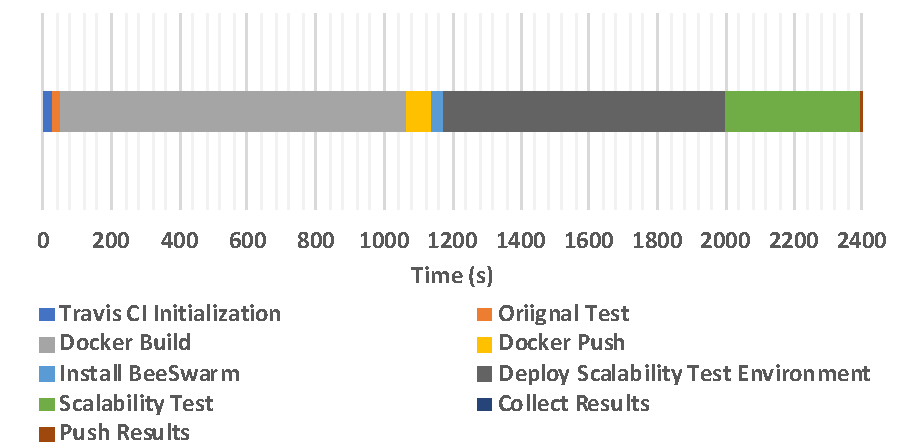
\includegraphics[width=0.5\textwidth]{figures/perf.pdf}
    \caption{Time breakdown of an example CI test with \texttt{BeeSwarm} scalability test.}
    \label{breakdown}
\end{figure}

\subsubsection{Scalability of \texttt{BeeSwarm} } % I think we don't need to separately 
\begin{figure}[h]
    \centering
    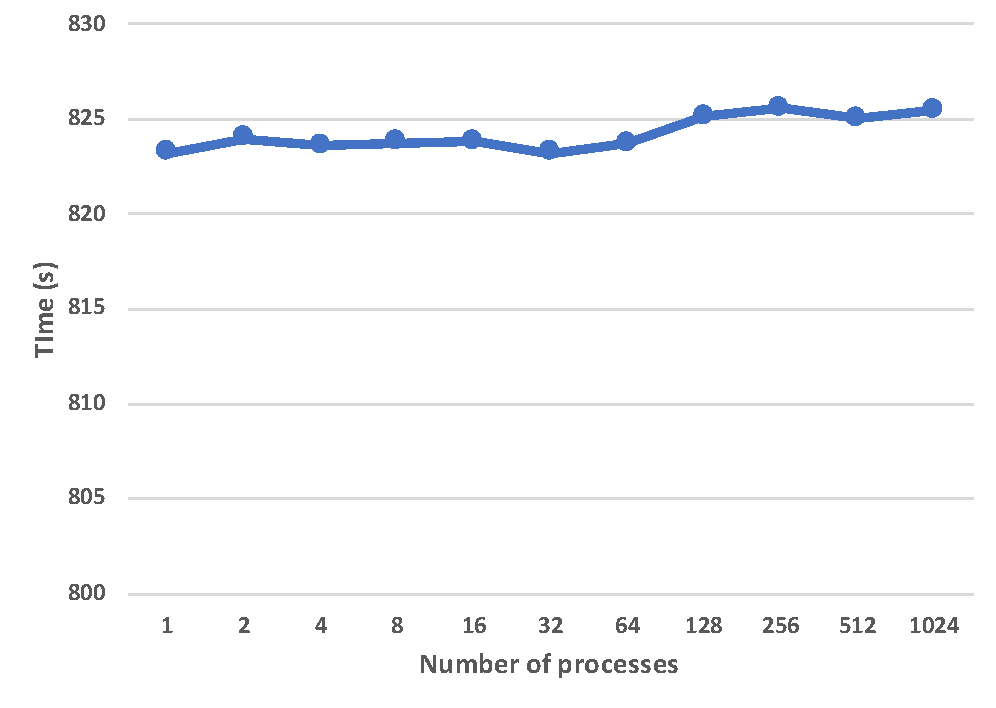
\includegraphics[width=0.45\textwidth]{figures/scalability.pdf}
    \caption{Scalability of deploying scalability test environment for \texttt{BeeSwarm}.}
    \label{scalability}
\end{figure}

Since BeeSwarm is designed for launching large-scaled parallel applications, the scalability of \texttt{BeeSwarm} itself is also very important. 
As we mentioned before, the main overhead of \texttt{BeeSwarm} comes from deploying the scalability test environment. \textbf{Fig. \ref{scalability}} shows the performance of deploying the scalability test environment for \texttt{BeeSwarm}. We test it with an increasing number of processes ranging from 1 to 1024. 
We run the scalability test on 16 instances on Chameleon cloud. Each instance has 64 cores. From \textbf{Fig. \ref{scalability}}, we can see the time cost is nearly constant (less than 900 seconds) as we increase the number of process. This indicate the scalability of \texttt{BeeSwarm} itself is very good.

%When the number of processes are greater than 64, \texttt{BeeSwarm} launches multiple instances. The time cost increases to about 1200 seconds and slightly increases with the number of instances. The sharp increase of time between launching one instance and two instances is because of the launching procedure of \texttt{BeeSwarm}. The scalability test environment that \texttt{BeeSwarm} deploys contains one master instance and zero or more worker instances. The master holds a working directory that is shared between workers, so the master instance must be launched first before workers. So, when we only need one instance only the master instance is launched. Otherwise, more worker instances need to be launched, taking extra time due to the dependency on the master instance. Beyond two instances, the time cost increases only slightly (4.9\% - 9.6\%, avg. 7.6\%). %\pat{you should probably quatify this here, what is slightly?}
%Worker instances do not have dependencies between each other, so they can be launched in parallel. The increase of time only comes from the extra configuration after each worker has launched.
%\texttt{BeeSwarm} shows good scalability performance on large scale scalability tests. %\pat{again should this be quantified?}

\subsection{Scalability Test Showcase}

\begin{figure}[h]
    \centering
    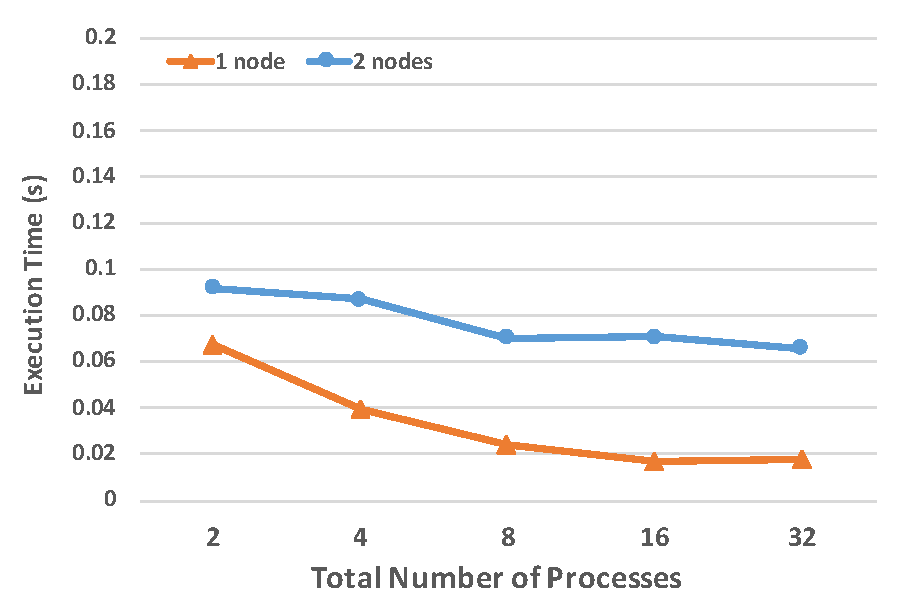
\includegraphics[width=0.45\textwidth]{figures/flecsale-result.pdf}
    \caption{The scalability test result of Flecsale.}
    \label{flecsale-result}
\end{figure}

We use Flecsale to showcase a sample scalability test using \texttt{BeeSwarm}. We configure it to run using 2 to 32 processes on one or two nodes. When using two nodes, we evenly divide the total number of processes among them (each has 1 to 16 processes). The file generated by \texttt{BeeSwarm} is in the comma separated values (CSV) file format, and we plotted the result data in \textbf{Fig. \ref{flecsale-result}}. %\trandles{Same comment here again about using colors on graphs}
Even with this simple test using \texttt{BeeSwarm}, we can observe some interesting behavior of Flecsale. We can see Flecsale gains better speedup (1.73x - 4.01x) on a single node environment compared to the speedup on two nodes (1.05x - 1.40x) given the same total number of processes. This may suggest that inter-node communication could be a performance bottleneck for Flecsale running on systems similar to Chameleon.


%However, the two node environment is more suitable for 64 processes compared to the single node.

This result can effectively give developers the scalability data of the application they are developing, so that they can make adjustment to their application in a more timely manner. Not only can the developer observe behavior of different processing schemes, but using \texttt{BeeSwarm} can help aid them to see performance improvement or degradation of their application as they push changes to the application. %\pat{I added the sentence before this comment} %\trandles{I worry that the claims about Flecsale scalability may be false given there's no discussion of interconnect, especially since you're using virtual machines.  Is this MPI or Legion using ethernet?  I don't think scalability will look like this on bare metal HPC nodes using IB or OPA with RDMA} %\pat{Can we make the point that this is an example and can't it be submitted to one of the other platforms?}
\section{Related Work}
\label{related_work}
Scalability is one of the most important metric we evaluate the quality of HPC applications. Many works have been done to build scalability test tools to facilitate HPC application development. For example, \cite{vetter2005mpip} proposed a a lightweight profiling library for MPI applications, which only based on statistical information about MPI functions and brings little performance overhead. \cite{chen2006stas} proposed a effective scalability testing and analysis system -- STAS. \cite{chung2006mpi} proposed a configurable MPI scalability analysis tool for Blue Gene/L supercomputer. \cite{brunst2013custom} proposed a performance too, Vampir, that can be used to detect hot spots in HPC applications. This can efficiently help HPC developers make their applications more scalable. \cite{merchant2012tool} proposed JACE (Job Auto-creator and Executor), a tool that enables automation of creation and execution of complex performance and scalability regression tests. It can help developers tune an application on a given platform to maximize performance given different optimization flags and turnable variables. \cite{muraleedharan2012hawk} presented a HPC performance and scalability test tool, Hawk-i, that uses cloud computing platforms to test HPC applications in order to reduce the effort to access relative scarce and on-demand high performance resources. \cite{bell2003paraprof} proposed, ParaProf, a portable, extensible, and scalable tool for parallel performance profile analysis. It gathers rich number of hardware counters and traceable information in order to offer much more detailed profiling result similar to state-of-the-art single process profiling tools. \cite{yoo2015patha} proposed a scalability test tool, PATHA, that uses system logs to extract key performance measures and apply the statistical tools and data mining methods on the performance data to identify bottlenecks or to debug the performance issues in HPC applications. Although these recent works are useful in scalability test for HPC applications, their tools or systems cannot be easily adopted by current HPC application development projects since they either require modification to the HPC application or complicated installation or configuration process in order to make their tools working properly on a given HPC platform. 

\section{Conclusions}
In this work, we first address the importance of the new in-situ analysis workflows. Next, we proposed \texttt{BeeFlow}, an in-situ analysis enabled workflow management system across HPC and cloud platforms with Docker support. We showed how we designed and optimized \texttt{BeeFlow} in the five-layer functionality architecture and evaluated the usability and performance. Moreover, we showcased three commonly used scientific workflows on \texttt{BeeFlow}. Finally, we compared \texttt{BeeFlow} with current existing workflow systems in multiple aspects and show that \texttt{BeeFlow} can be easily adopted to launch modern in-situ workflows in our case studies. Comparisons also showed that \texttt{BeeFlow} brings much better usage complexity and user time cost compared with manual approach and similar results compared to existing commonly used workflow tools. 



%\patg{This just tells what you did you should also state what the comparisons todl you in a concise manner, why use BeeFlow?}


\section{Acknowledgement}
This work was funded by the the US Government contract DE-AC52-06NA25396 for Los Alamos National Laboratory, operated by Los Alamos National Security,
LLC, for the US Department of Energy. This work was also supported by NSF Award No. 1513201. Results presented in this paper were obtained using the Chameleon Cloud sponsored by the National Science Foundation. The publication has been assigned the LANL identifier LA-UR-18-27912.
\bibliographystyle{ACM-Reference-Format}
\bibliography{biblio}
\end{document}


